\chapter{Perancangan}
\label{chap:perancangan}


Pada bab ini dijelaskan mengenai perancangan aplikasi yang dibangun meliputi perancangan kelas algoritma pendeteksi gerakan kepala, \textit{GameObject},  \textit{Gameplay}, dan perancangan antarmuka.

\section{Perancagan Kelas Algoritma Pendeteksi Gerakan Kepala}
\label{sec:perancangan_kelas_algoritma_Pendeteksi_Gerakan_Kepala}

Pada subbab \ref{sec:analisis_metode_pendeteksi_gerakan_kepala} telah dijelaskan algoritma pendeteksi gerakan kepala secara prosedural. Untuk merapihkan algoritmanya, dibuatlah diagram kelas rinci untuk memenuhi kebutuhan dalam pembangunan aplikasi. Desain diagram kelas ini pada dasarnya membagi  masalah-masalah pada algoritma di subbab \ref{sec:analisis_metode_pendeteksi_gerakan_kepala} menjadi masalah-masalah yang lebih sederhana. Kemudian setiap masalah disatukan kembali untuk menyelesaikan masalah pendeteksian kepala. Deskripsi kelas beserta fungsi dari diagram kelas dijelaskan sebagai berikut:

\begin{figure}[htbp]
\centering
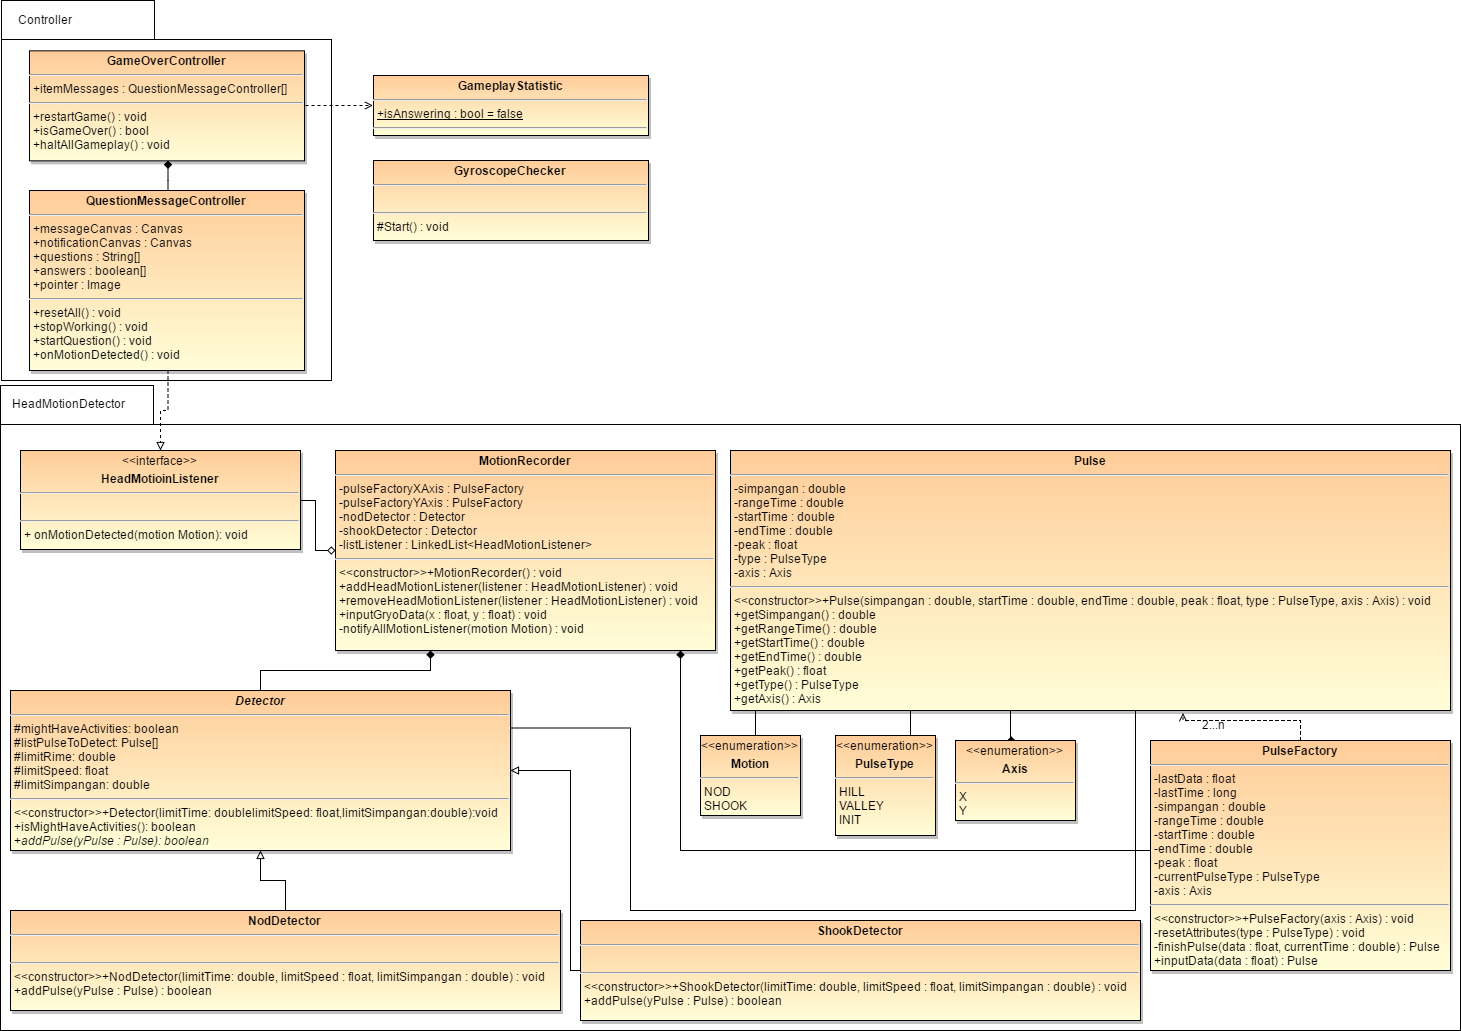
\includegraphics[scale=0.6]{Gambar/diagram-kelas-algoritma-pendeteksi-gerakan-kepala.png}
\caption{Diagram Kelas Algoritma Pendeteksi Gerakan Kepala. (Gambar diputar sembilan puluh derajat searah jarum jam)}
\label{fig:diagram-kelas-algoritma-pendeteksi-gerakan-kepala}
\end{figure}

\begin{itemize}
    \item Kelas GameplayStatistic\\
    Kelas ini bertujuan untuk menyimpan seluruh atribut-atribut statis pada keseluruhan permainan. Saat ini kelas ini hanya menyimpan atribut isAnswered saja, yang mengindikasikan bahwa suatu pertanyaan yang telah muncul telah dijawab. 
    \item Kelas GyroscopeChecker\\
    Kelas ini digunakan untuk mengecek apakah perangkat yang sedang menjalankan permainan ini memiliki sensor gyroscope. Kelas ini tidak memiliki hubungan kepada kelas lain karena kelas ini berjalan pada Scene yang berbeda dengan kelas lainnya. Pengecekan perangkat dilakukan pada saat aplikasi mulai dijalankan, oleh karena itu implementasi pengecekan perangkat terletak pada method Awake().
    \item Package Controller
    \begin{itemize}
        \item Kelas GameOverController\\
        Kelas ini bertujuan untuk mendeteksi kondisi \textit{game over} dan menampilkan pesan \textit{game over}.
        Atribut-atribut pada kelas ini adalah sebagai berikut:
        \begin{itemize}
            \item public QuestionMessageController[] itemMessages\\
            Atribut ini digunakan untuk menyimpan seluruh QuestionMessageController yang ada pada permainan agar dapat diberhentikan dan diatur ulang.
        \end{itemize}
        Method-method pada kelas ini adalah sebagai berikut:
        \begin{itemize}
            \item public void restartGame()\\
            Method ini berfungsi untuk mengembalikan kondisi permainan ke kondisi awal, untuk mengulang permainan jika permainan telah selesai.
            \item public boolean isGameOver()\\
            Method ini berfungsi untuk mengecek apakah permainan sudah selesai atau belum. Method ini dipanggil secara berulang-ulang setiap satu \textit{frame} pada permainan.
            \item public void haltAllGameplay()\\
            Method ini berfungsi untuk memberhentikan seluruh fungsi permainan. Method ini dipanggil ketika permainan telah selesai.
        \end{itemize}
        \item Kelas QuestionMessageController\\
        Kelas ini digunakan untuk mengatur tampilan pesan pertanyaan pada permainan. Kelas ini juga mengatur kondisi permainan bergantung dari masukan pengguna, yaitu anggukan dan gelengan kepala.
        Atribut-atribut pada kelas ini adalah sebagai berikut.
        \begin{itemize}
            \item public Canvas messageCanvas\\
            Atribut ini digunakan untuk mendapatkan Canvas yang menampilkan pesan pertanyaan kepada pengguna.
            \item public Canvas notificationCanvas\\
            Atribut ini digunakan untuk mendapatkan Canvas yang menampilkan pesan pemberitahuan kepada pengguna.
            \item public String[] question\\
            Atribut ini digunakan untuk menyimpan pertanyaan-pertanyaan yang ditampilkan pada messageCanvas.
            \item public boolean[] answers\\
            Atribut ini digunakan untuk menyimpan jawaban-jawaban penentu untuk setiap pertanyaan yang ada.
            \item public Image pointer\\
            Atribut ini digunakan untuk mendapatkan gambar yang digunakan sebagai pengukur kondisi permainan.
        \end{itemize}
        Method-method pada kelas ini adalah sebagai berikut:
        \begin{itemize}
            \item public void resetAll()\\
            Method ini berfungsi untuk mengembalikan kondisi permainan menjadi kondisi awal permainan.
            \item public void stopWorking()\\
            Method ini berfungsi untuk memberhentikan semua fungsi pada suatu objek QuestionMessageController.
            \item public void startQuestion()\\
            Method ini berfungsi untuk memulai atau memunculkan suatu pertanyaan pada tampilan.
            \item public void onMotionDetected(Motion motion)\\
            Method ini dipanggil jika terdeteksi suatu gerakan kepala. Parameter motion diisi dengan spesifikasi gerakan yang terdeteksi.
        \end{itemize}
    \end{itemize}
    \item Package HeadMotionDetector
    \begin{itemize}
        \item interface HeadMotionListener\\
        Interface ini di-\textit{implement} oleh kelas-kelas yang menggunakan hasil dari pendeteksian gerakan kepala.
        Method-method abstrak pada interface ini adalah sebagai berikut:
        \begin{itemize}
            \item public void onMotionDetected(Motion motion)\\
            Method ini dipanggil oleh jika terdeteksi suatu gerakan kepala. Parameter motion diisi dengan spesifikasi gerakan yang terdeteksi.
        \end{itemize}
        \item Kelas MotionRecorder\\
        Kelas ini digunakan untuk merekam, menentukan, dan mendeteksi gerakan kepala. 
        Atribut-atribut pada kelas ini adalah sebagai berikut:
        \begin{itemize}
            \item private PulseFactory pulseFactoryXAxis\\
            Atribut ini digunakan untuk menyimpan PulseFactory yang merekam data gyroscope pada sumbu X.
            \item private PulseFactory pulseFactoryYAxis\\
            Atribut ini digunakan untuk menyimpan PulseFactory yang merekam data gyroscope pada sumbu Y.
            \item private Detector nodDetector\\
            Atribut ini digunakan untuk menyimpan Pendeteksi gerakan mengangguk.
            \item private Detector shookDetector\\
            Atribut ini digunakan untuk menyimpan Pendeteksi gerakan menggeleng.
            \item private LinkedList<HeadMotionListener> listListener\\
            Atribut ini digunakan untuk menyimpan kelas-kelas yang menjadi \textit{listener} pendeteksi gerakan kepala.
        \end{itemize}
        Method-method pada kelas ini adalah sebagai berikut:
        \begin{itemize}
            \item public MotionRecorder() \\
            Constructor ini digunakan untuk menginisialisasi atribut-atribut yang digunakan.
            \item public void addHeadMotionListener(HeadMotionListener listener)\\
            Method ini digunakan untuk menambahkan \textit{listener} baru pada atribut listListener
            \item public void removeHeadMotionListener(HeadMotionListener listener)\\
            Method ini digunakan untuk menghapus suatu listener pada atribut listListener.
            \item public void inputGyroData(float x, float y) \\
            Method ini digunakan untuk memasukkan data gyroscope yang digunakan untuk mendeteksi gerakan mengangguk dengan menggeleng.
            \item public void notifyAllMotionListener(Motion motion) \\ 
            Method ini memberitahu seluruh \textit{listener} ketika terdeteksi suatu gerakan. Jenis gerakan yang diberitahukan adalah jenis gerakan pada parameter tersebut.
        \end{itemize}
        \item Kelas PulseFactory\\
        Kelas ini berguna untuk mendeteksi \textit{Pulse} yang terjadi pada grafik data gyroscope. Beberapa atribut yang dimiliki oleh kelas ini menjadi kriteria dari suatu \textit{Pulse} yang terdeteksi.
        Atribut-atribut tersebut adalah:
        \begin{itemize}
            \item private float lastData\\
            Atribut ini menyimpan data sebelum data yang baru dimasukkan
            \item private float lastTime\\
            Atribut ini menyimpan waktu pada pemasukkan data sebelum daya yang baru dimasukkan.
            \item private double simpangan\\
            Atribut ini menyimpan simpangan terjauh pada \textit{Pulse} terakhir yang terdemeteksi.
            \item private double rangeTime\\
            Atribut ini menyimpan rentang waktu yang terjadi pada suatu \textit{Pulse}
            \item private double startTime\\
            Atribut ini menyimpan waktu mulai dari suatu \textit{Pulse} yang terjadi.
            \item private double endTime\\
            Atribut ini menyimpan waktu akhir dari suatu \textit{Pulse} yang terjadi.
            \item private float peak\\
            Atribut ini menyimpan puncak nilai tertinggi atau terendah dari suatu \textit{Pulse} bukit atau lembah.
            \item private PulseType\\
            Atribut ini menyimpan tipe \textit{Pulse} antara bukit atau lembah.
            \item private Axis axis\\
            Atribut ini mendefinisikan sumbu yang direkam datanya.    
        \end{itemize}
        Method-method pada kelas ini adalah:
        \begin{itemize}
            \item public PulseFactory(Axis axis)\\
            Constructor ini berfungsi untuk mendefinisikan sumbu pada gyroscope yang dideteksi.
            \item private void resetAttributes()\\
            Method ini berfungsi untuk mengembalikan nilai-nilai atribut kembali ke nilai asal.
            \item private Pulse finishPulse(float data, double currentTime)\\
            Method ini dipanggil ketika grafik melewati angka nol. Pada pemanggillan ini \textit{Pulse} baru terdeteksi dan resetAttributes() dipanggil untuk pendeteksian \textit{Pulse} selanjutnya.
            \item public Pulse inputData(float data)\\
            Method ini digunakan untuk memasukkan data gyroscope baru.
        \end{itemize}
        \item Kelas Detector\\
        Kelas ini merupakan kelas yang mendefinisikan pendeteksi gerakan kepala. Sub-class kelas ini adalah NodDetector dengan ShookDetector
        Atribut-atribut pada kelas ini adalah:
        \begin{itemize}
            \item public Detector(float limitSpeed, double limitSimpangan)\\
            Constructor ini digunakan untuk meninisialisasi batasan-batasan yang didefinisikan pada atribut-atribut kelas ini.
            \item protected boolean mightHaveActivities()\\
            Atribut ini menunjukkan apakah suatu detector memiliki kemungkinan sedang mendeteksi gerakan atau tidak.
            \item protected Pulse[] listPulseToDetect()\\
            Atribut ini menyimpan beberapa \textit{Pulse} untuk diperiksa karakteristiknya, apakah sesuai dengan algoritma pendeteksian gerakan kepala.
            \item protected float limitSpeed()\\
            Atribut ini mendefinisikan batas kecepatan angular yang sesuai dengan pendeteksian gerakan kepala.
            \item protected double limitSimpangan()\\
            Atribut ini mendefinisikan batas Simpangan yang sesuai dengan pendeteksian gerakan kepala.
        \end{itemize}
        \item Kelas NodDetector dengan ShookDetector\\
        Kelas ini berisi algoritma untuk mendeteksi gerakan mengangguk atau menggeleng. Kelas ini merupakan turunan dari kelas Detector
        \item Kelas Pulse\\
        Kelas ini digunakan hanya untuk menyimpan karakteristik-karakteristik dari suatu \textit{Pulse} yang terbentuk oleh kelas PulseDetector. Atribut-atribut pada kelas ini serupa dengan atribut-atribut pada kelas PulseDetector. Method-method pada kelas ini hanyalah Getter dengan Constructor saja.  
    \end{itemize}
\end{itemize}


\section{Perancangan Hierarki GameObject pada Unity}
\label{sec:perancangan_hierarki_gameobject_pada_unity}

Perancangan hierarki pada Unity merupakan salah satu perancangan yang cukup penting. Perancangan ini penting karena mempermudah pencarian, pemilihan, perubaha transformasi GameObject pada dunia permainan yang sedang dibuat. Selain itu perancangan ini dapat membantu pengguna Unity untuk membuat suatu GameObject yang memiliki sifat relatif terhadap suatu GameObject yang lain. Oleh Karena itu perancangan hierarki dibahas pada subbab ini.

Permainan ini hanya dibangun dengan menggunakan dua buah scene saja. Scene pertama digunakan hanya untuk mengecek apakah perangkat memiliki sensor gyroscope atau tidak. Scene kedua digunakan untuk implementasi keseluruhan permainan. Permainan ini tidak memerlukan Scene yang banyak karena permainan ini hanya memiliki satu ruangan saja. Sebagian besar pada perancangan ini hanyalah mengelompokkan GameObject-GameObject pada Scene. Perancangan hierarki scene pertama hanyalah satu buah GameObject GryoscopeChecker saja. Gambar \ref{fig:perancangan_hierarki_game_object} merupakan hasil dari perancangan hierarki Scene kedua permainan ini.
\begin{figure}[hbtp]
\dirtree{%
	.1 {Player}.
	.2 {Main Camera}.
	.3 {GvrReticlePointer}.
	.3 {GvrCanvas}.
	.4 {Game Over UI}.
	.1 {Gameplay Canvas}.
	.2 {Panel}.
	.2 {Pointer}.   
	.2 {HUD}.
	.1 {Room}.
	.2 {Desk Chair}.
	.2 {Table}.
	.2 {Ceiling}.
	.2 {Door}.
	.2 {Walls}.
	.2 {Floor}.
	.2 {Writing Board}.
	.2 {Desk Lamp}.
	.2 {Light Switch}.
	.1 {Items}.
	.2 {Notebook}.
	.3 {ItemMessageController}.
	.4 {Notification Canvas}.
	.5 {Text}.
	.4 {ItemMessage Canvas}.
	.5 {Panel}.
	.5 {Text}.
	.2 {Telephone}.
	.3 {ItemMessageController}.
	.2 {Pencil}.
	.2 {Pencil Holder}.
	.2 {Photo Frame}.
}
\caption{Perancangan hierarki Game Object}
\label{fig:perancangan_hierarki_game_object}
\end{figure}

Pada Perancangan di atas ada beberapa GameObject utama, diantaranya adalah Player, GameplayCanvas, Room, dan Items. GameObject Player digunakan sebagai camera pada dunia permainan tersebut. Camera pada Player ini bergerak mengikuti orientasi pada \textit{smartphone}. Pada GameObject ini terdapat GameObject Main Camera yang berfungsi untuk menjadi kamera pada permainan dan menentukan titik pandang pengguna. Main Camera memiliki dua buah \textit{Child} Game Object. Kedua GameObject tersebut adalah GvrReticlePointer dan GameOverCanvas. GvrReticlePointer berguna untuk menampilkan titik pandang pengguna. GvrReticlePointer ini menjadi lingkaran ketika objek yang dipandangnya dapat memberikan respons dari masukan tombol pada Google Cardboard. GameOverCanvas berguna untuk menampilkan pesan "Game Over!" ketika permainan berakhir.

GameObject GameplayCanvas digunakan untuk menunjukkan kondisi permainan sekarang. GameObject ini memiliki dua buah child yaitu Panel, Pointer, dan HUD. Panel berfungsi sebagai bidang putih pada UI. Pointer berfungsi sebagai menunjuk kondisi permainan pada saat ini. HUD adalah bentuk kurang lebih 1/6 lingkaran yang membatasi Pointer. 

GameObject Room digunakan untuk menyimpan model-model dekorasi dalam ruangan. \textit{Child} dari GameObject hanya merupakan model-model tiga dimensi yang membentuk ruangan pada dunia game.

GameObject Item digunakan untuk menyimpan model-model barang yang ada pada ruangan. Sebagian GameObject pada Item memiliki component yang diberikan script untuk mendeteksi gerakan kepala. GameObject yang diberikan script tersebut adalah GameObject yang memiliki \textit{Child} GameObject ItemMessageController, yaitu Notebook dengan Telephone. Selain kedua GameObject tersebut GameObject lainnya merupakan model-model dekorasi pada meja.

\section{Perancangan \textit{Gameplay} dan Perancangan Antarmuka}
\label{sec:perancangan_gameplay}

Permainan ini merupakan permainan yang pemainnya berperan sebagai pemimpin dari suatu perusahaan. Tugas dari permainan ini adalah memilih pilihan-pilihan yang sesuai dari kondisi yang sedang terjadi. Pemain diberi pertanyaan dalam mengatur perusahaan tersebut. Pertanyaan tersebut hanya dapat dijawab ya atau tidak. Jawaban ya dilakukan dengan mengangguk dan jawaban tidak dengan menggeleng. Jawaban yang mengacu untuk menguntungkan perusahaan membuat tingkat kesenangan karyawan berkurang. Jawaban yang mengacu untuk menyenangkan karyawan merugikan perusahaan.

Takaran kesenangan karyawan dengan keuntungan perusahaan digambarkan dengan meteran seperti pada gambar \ref{fig:meteran_permainan}. Jika jarum pada meteran tersebut mengarah ke kiri, berarti karyawan perusahaan sedang memiliki tingkat kesenangan yang tinggi, namun perusahaan tidak mendapatkan keuntungan yang baik. Begitu pula sebaliknya jika jarum mengarah ke kanan. 

\begin{figure}[htbp]
\centering
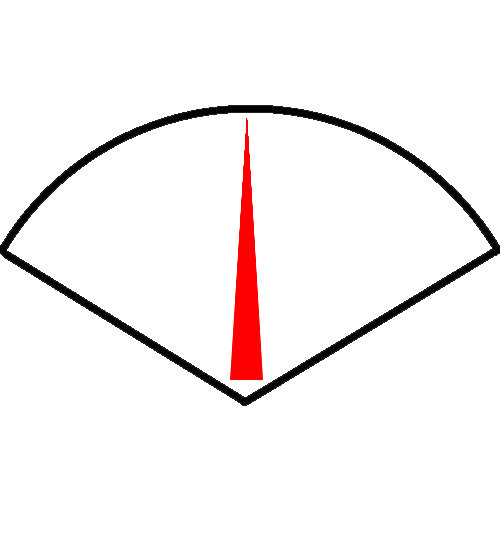
\includegraphics[scale=0.3]{Gambar/HUDBar.png}
\caption{Meteran pada permainan.}
\label{fig:meteran_permainan}
\end{figure}

Tidak ada kondisi menang pada permainan ini, karena permainan ini terus berlangsung hingga pemain kalah. Pemain kalah jika meteran terlalu mengarah ke kiri, atau terlalu mengarah ke kanan. Ketika pemain sudah kalah, muncul pesan "Game Over!" (Gambar \ref{fig:desain_pop_up}). Jika pemain menarik atau menekan tombol pada Google Cardboard-nya, permainan dimulai kembali dari awal. 

Antarmuka yang ditampilkan pada permainan ini merupakan pemandangan seseorang pemimpin perusahaan (Pemain) pada meja kerjanya. Ruangan tersebut sangat sederhana, yaitu ruangan dengan bentuk balok biasa dan diisi dengan beberapa model untuk dekorasi. Pada meja kerja terdapat beberapa alat seperti, pensi, buku catatan, telepon, lampu, dan lain sebagainya. Alat-alat yang ditambahkan \textit{script} C\# untuk dapat mendeteksi anggukan dan gelengan adalah telepon dan buku catatan. Ruangan tersebut digambarkan pada gambar \ref{fig:gambar_desain_ruangan}.

\begin{figure}[htbp]
\centering
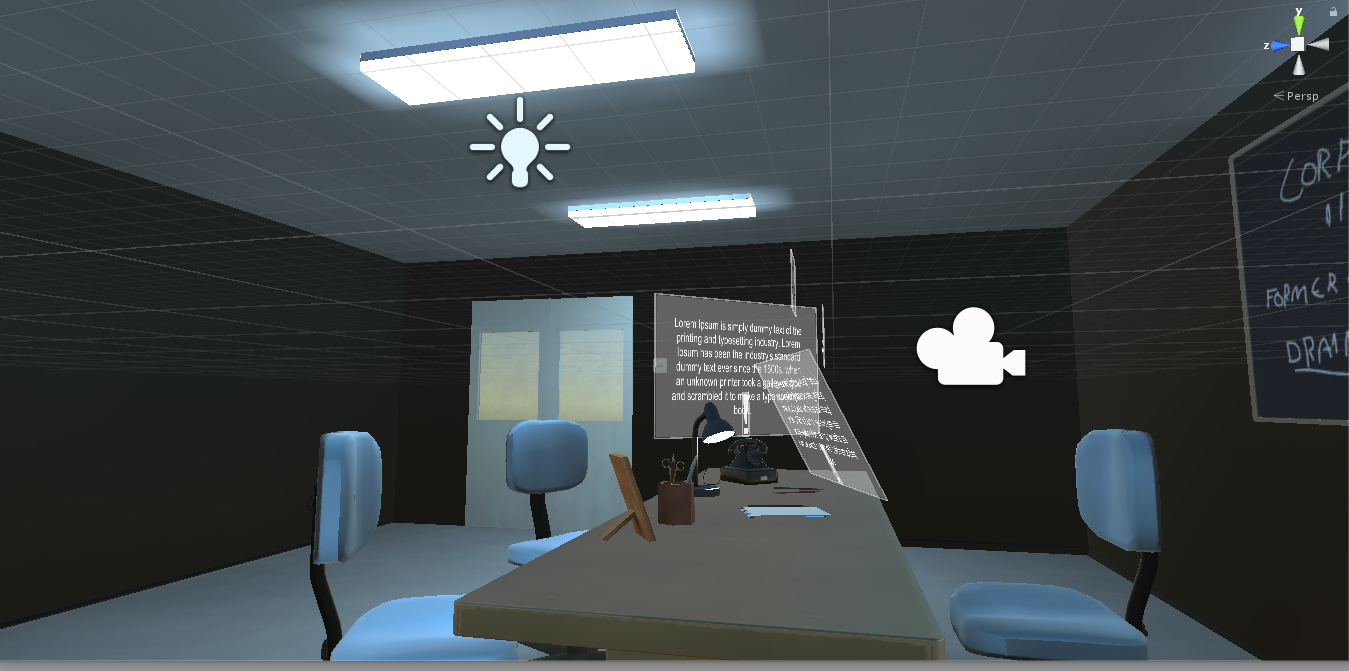
\includegraphics[scale=0.3]{Gambar/Desain-ruangan.PNG}
\caption{Desain ruangan untuk permainan yang dibuat.}
\label{fig:gambar_desain_ruangan}
\end{figure}

Unity Asset Store menyediakan berbagai macam aset seperti \textit{model}, \textit{texture}, \textit{prefab}, animasi, bahkan \textit{scripts}. Perancangan aplikasi ini menggunakan beberapa aset yang diperoleh dari Unity Asset Store. Tabel \ref{tab:tabel_aset_yang_digunakan} adalah aset-aset yang digunakan pada perancangan antar muka ini.

Untuk menampilkan pertanyaan, pemain harus menunggu suatu alat menampilkan notifikasi yang ditunjukkan dengan memunculkan karakter tanda seru (!) di atas alat tersebut. Ketika notifikasi tersebut muncul, pemain dapat menghadapkan pandangannya ke alat tersebut dan menarik/menekan tombol pada Google Cardboard untuk menampilkan pertanyaan yang diberikan. Pertanyaan yang diberikan diberikan dengan memunculkan suatu \textit{pop-up} di atas alat tersebut yang ditulis pertanyaan yang ditanyakan (Notifikasi dan \textit{pop-up} ditunjukkan pada gambar \ref{fig:desain_pop_up}). Jumlah pertanyaan yang dapat dimunculkan hanyalah satu pertanyaan saja, tidak dapat memunculkan dua buat pertanyaan secara bersamaan. Setelah pertanyaan dijawab dengan anggukan atau gelengan \textit{pop-up} tersebut menghilang, dan meteran bergerak tergantung dari jawaban pemain.

\begin{table}[htbp]
    \centering
    \begin{tabular}{|p{1cm}||p{6cm}|p{6cm}|}
    \hline\\
    \hline
       No & Nama Aset & Penerbit \\
    \hline
        1 &  Morgue Room PBR \footnote{https://www.assetstore.unity3d.com/en/\#!/content/65817} & Rokay3D\\
    \hline
        2 &  Old Telephone \footnote{https://www.assetstore.unity3d.com/en/\#!/content/62434} & Rokay3D\\
    \hline
        3 &  Native Popups for iOS and Android \footnote{https://www.assetstore.unity3d.com/en/\#!/content/29566} & The Next Flow\\
    \hline
    \end{tabular}
    \caption{Tabel Aset-aset yang digunakan.}
    \label{tab:tabel_aset_yang_digunakan}
\end{table}

\begin{figure}[htbp]
\centering
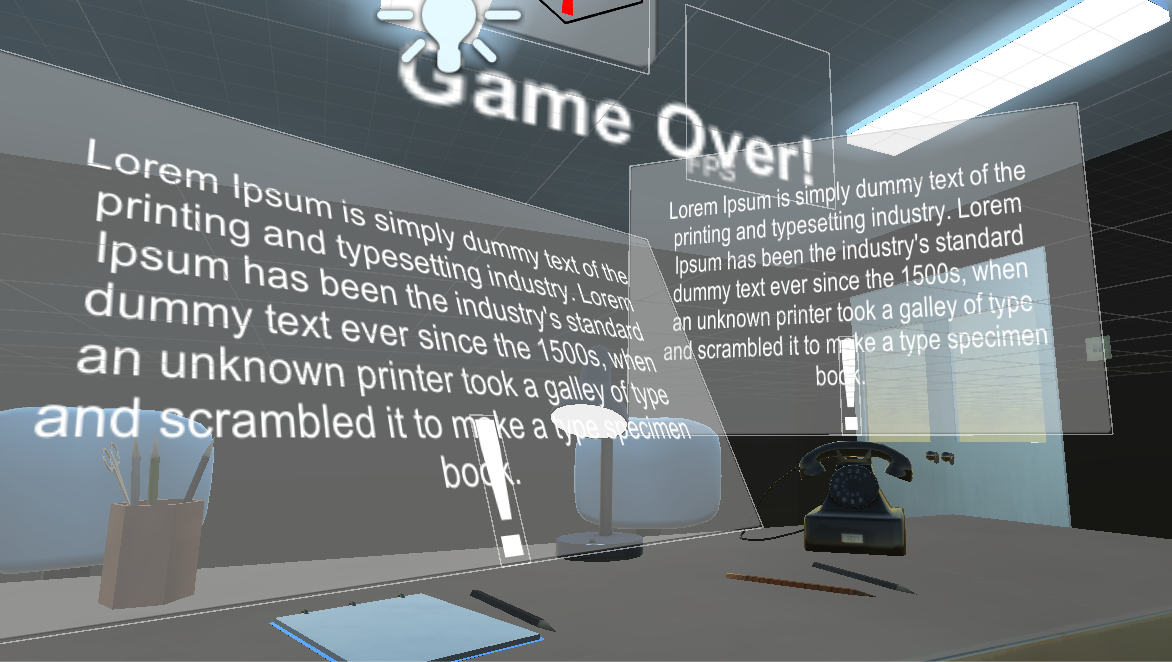
\includegraphics[scale=0.3]{Gambar/desain-pop-up.PNG}
\caption{Desain User Interface}
\label{fig:desain_pop_up}
\end{figure}
